\section{Evaluierung}

\begin{frame}{\insertsection}
  \begin{block}<+->{Versuchsaufabau}
    \begin{itemize}
        \item Versuchsperson bewegt sich mit dem Handy auf den Hauptcampus
        \item Strecke ist festgelegt ($x^{\text{truth}}, x^{\text{truth*}}$)
        \item 186 von 742 GPS-Daten wurden als fehlerhaft festgestellt
    \end{itemize}
  \end{block}
    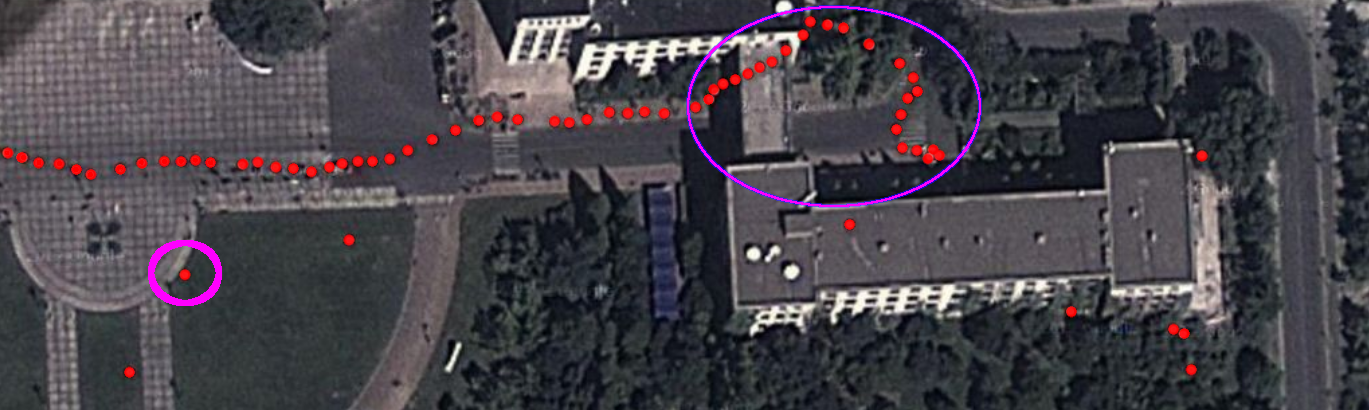
\includegraphics[width=\textwidth]{GPS_Motivation_Example.png}
\end{frame}

\subsection{Ordnung}

\begin{frame}{\insertsubsection}
\begin{figure}[htbp]
    \centering
    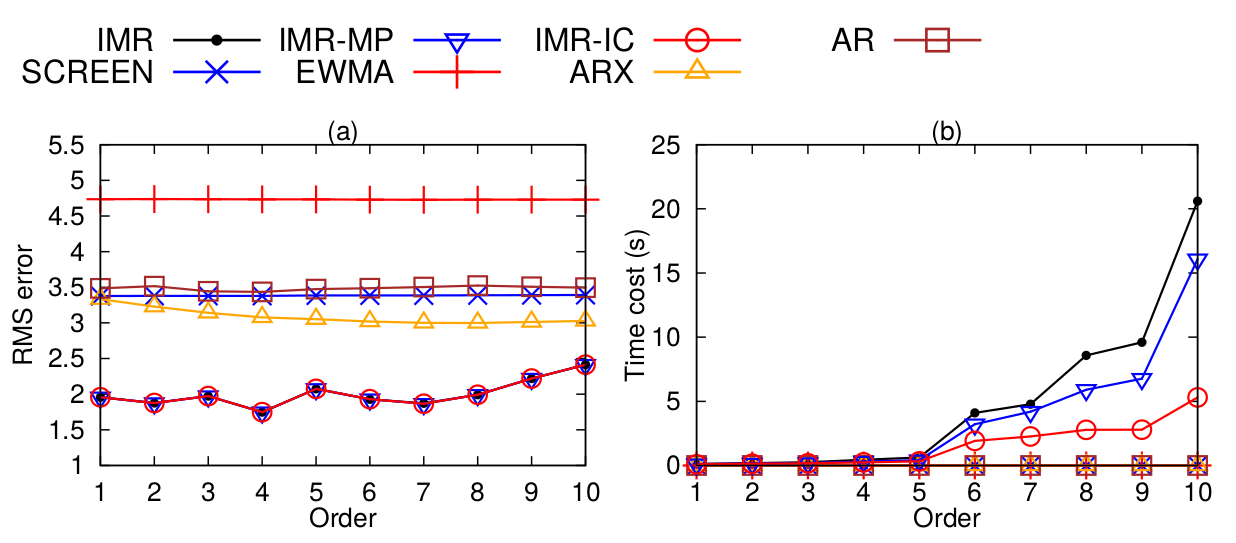
\includegraphics[width=\textwidth]{../plots/varying_order_p.png}
    \caption{Unterschiedliche Ordnung $p$ �ber GPS-Daten mit $\tau$ = 0.2, Datengr��e 750 und Markierungsrate 0.2}%
    \label{varying_order_p}
\end{figure}
\end{frame}

\subsection{Schwellenwert}

\begin{frame}{\insertsubsection}
\begin{figure}[htbp]
    \centering
    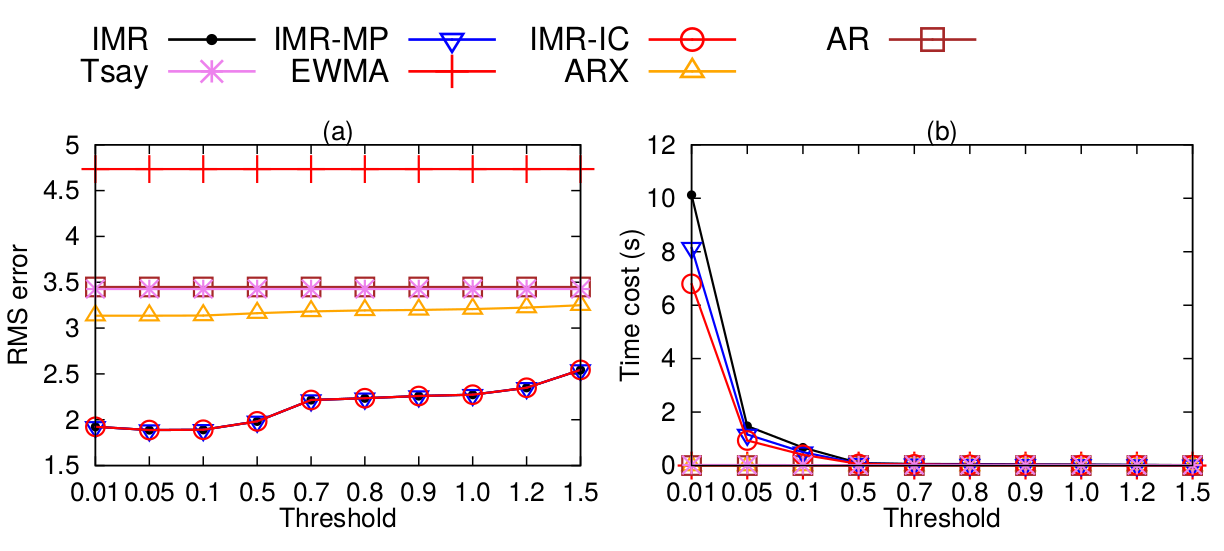
\includegraphics[width=\textwidth]{../plots/varying_threshold.png}
    \caption{Unterschiedliche Schwellenwerte $\tau$ �ber GPS-Daten mit $p$ = 3, Datengr��e 750 und Markierungsrate 0.2}%
    \label{varying_threshold}
\end{figure}
\end{frame}

\subsection{Maximale Anzahl von Iterationen}

\begin{frame}{\insertsubsection}
\begin{figure}[htbp]
    \centering
    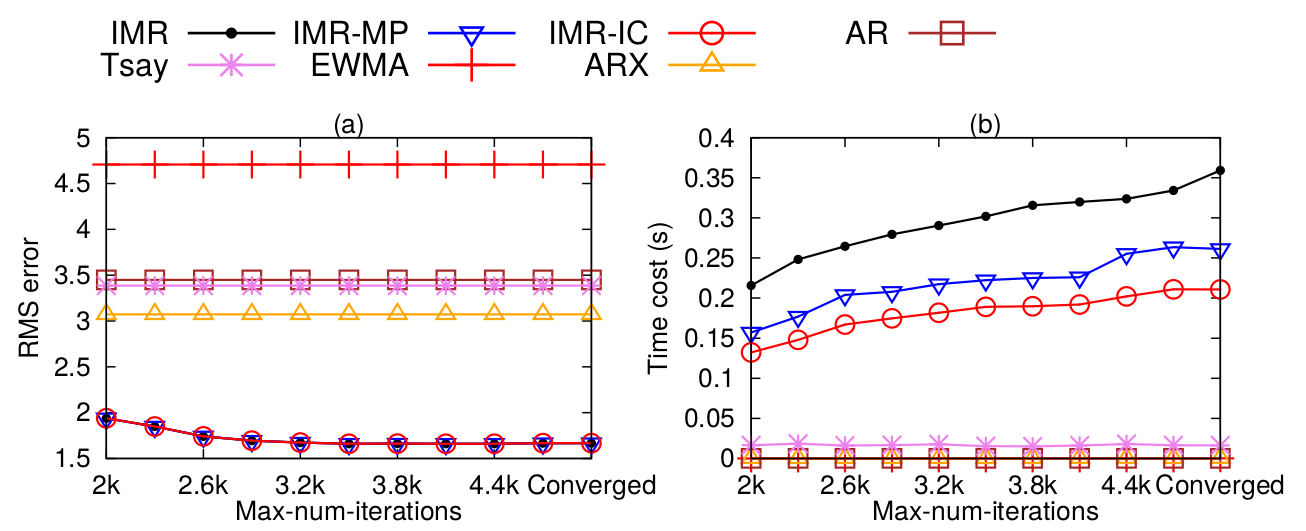
\includegraphics[width=\textwidth]{../plots/varying_maximum_number.png}
    \caption{Unterschiedliche maximale Anzahl von Iterationen �ber GPS-Daten mit $\tau = 0,2$, $p$ = 3 und Datengr��e 750}%
    \label{varying_maximum_number}
\end{figure}
\end{frame}

\subsection{Markierungsrate}

\begin{frame}{\insertsubsection}
\begin{figure}[htbp]
    \centering
    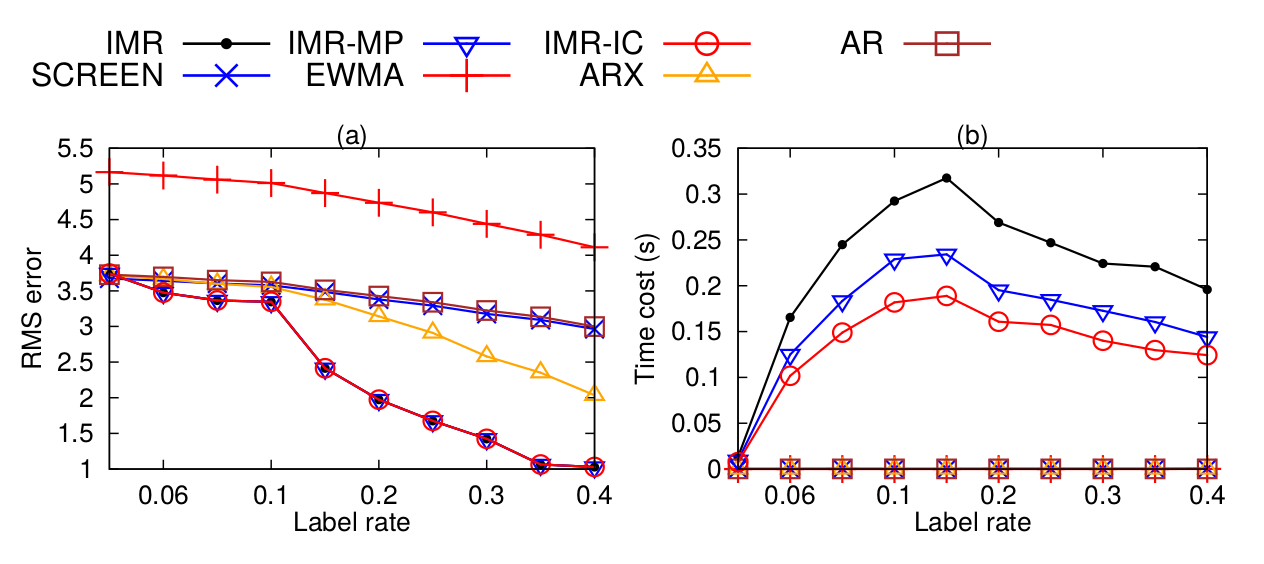
\includegraphics[width=\textwidth]{../plots/varying_labeling_rate.png}
    \caption{Unterschiedliche Markierungsraten �ber GPS-Daten mit $\tau = 0,2$, $p$ = 3 und Datengr��e 750}%
   \label{varying_labeling_rate}
\end{figure}
\end{frame}
